% IEEE GRSL letter — revision R2 (GRSL-01920-2026)
% Environment-Conditioned Score Thresholding for Clutter-Invariant False-Alarm Operation of Deep SAR Ship Detectors
\documentclass[journal]{IEEEtran}

% ---- Preamble ----
\usepackage{graphicx}
\usepackage{amsmath}
\usepackage{amssymb}
\usepackage{booktabs}
\usepackage{array}
\usepackage{subcaption}
\usepackage[hidelinks]{hyperref}
\usepackage{enumitem}
\usepackage{tikz}
\usepackage{xcolor}
\usetikzlibrary{shapes.geometric, arrows.meta, positioning}

% Remaining placeholders are printed in blue; replace before final compile.
\newcommand{\TBD}[1]{\textcolor{blue}{#1}}
\providecommand{\linelabel}[1]{}

\IEEEpubidadjcol

\renewcommand{\topfraction}{0.95}
\renewcommand{\bottomfraction}{0.95}
\renewcommand{\textfraction}{0.05}
\renewcommand{\floatpagefraction}{0.75}
\setcounter{topnumber}{3}
\setcounter{bottomnumber}{2}
\setcounter{totalnumber}{5}

\begin{document}

\title{Environment-Conditioned Score Thresholding for Clutter-Invariant False-Alarm Operation of Deep SAR Ship Detectors}

\author{Songtao~Hu,~\IEEEmembership{}
        Liang~Chen,~\IEEEmembership{}
        Qianyue~Zhang,~\IEEEmembership{}
        and~Wenchao~Liu$^{*}$,~\IEEEmembership{}
\thanks{S.~Hu, L.~Chen, and W.~Liu are with the School of Information
and Electronics, Beijing Institute of Technology, Beijing 100081, China.
S.~Hu and Q.~Zhang are also with the China Academy of Electronics and
Information Technology, Beijing 100041, China.
Emails: \texttt{3420215015@bit.edu.cn} (S.H.),
\texttt{chenl@bit.edu.cn} (L.C.),
\texttt{qianyue19990505@gmail.com} (Q.Z.),
\texttt{6120220028@bit.edu.cn} (W.L., corresponding author).}}

\maketitle

\begin{abstract}
\linelabel{ln:abs}Deep SAR ship detectors are deployed with one global confidence
threshold, although sea clutter changes their post-NMS score distribution
from scene to scene. The false-alarm rate delivered by a fixed threshold
therefore varies with clutter: on SARDet-100K and SAR-Ship-Dataset, a
YOLOv8s detector at $T{=}0.40$ produces 5--6 times more false alarms per
image in the high-clutter tertile than in the low-clutter one. In the
spirit of constant-false-alarm-rate (CFAR) detection, we study a
training-free threshold policy $T(e)$ that maps a per-image clutter
proxy $e$ --- the standard deviation of background grey levels outside
detector boxes --- to a per-stratum threshold calibrated offline to a
false-alarm budget or a precision target. At the false-alarm budget of
$T{=}0.40$, $T(e)$ reduces the cross-stratum spread of false alarms per
image by $4.5\times$ (SARDet-100K) and $41\times$ (SAR-Ship-Dataset); over
twelve pre-specified dataset--target settings the reduction is
$2.8$--$41\times$ and its bootstrap 95\,\% interval always excludes zero.
Neither a global threshold fitted to the same target nor a random-binning
placebo achieves this. The price is $-1.6$ to $+0.6$~pp F1. Controls also
show that when $T(e)$ instead maximizes F1, its small aggregate gain
equals that of a validation-tuned global threshold. The proxy tracks
image-level clutter statistics (Spearman $\rho{=}0.91$--$0.92$ with mean
backscatter).\linelabel{ln:absend}
\end{abstract}

\begin{IEEEkeywords}
SAR ship detection, constant false alarm rate, score thresholding, sea
clutter, operating point calibration, SARDet-100K, SAR-Ship-Dataset.
\end{IEEEkeywords}

% ---------------------------------------------------------------
\section{Introduction}
\label{sec:intro}
% ---------------------------------------------------------------

Synthetic aperture radar (SAR) is a primary modality for maritime
surveillance because it is independent of cloud cover and
daylight~\cite{brusch2011}. \linelabel{ln:sota}Recent deep SAR ship
detectors, including YOLO-based models~\cite{yolov8,sun2021bifa}, perform
strongly in complex and cluttered maritime
scenes~\cite{li2022survey,sardet100k,sarship2019}, yet a gap to simple
scenes remains: BiFA-YOLO reports F1 $0.959$ offshore but $0.922$ in
inshore scenes with land interference~\cite{sun2021bifa}, and inshore
detection is likewise weaker on SSDD~\cite{zhang2021ssdd,zhang2022bslm}.\linelabel{ln:sotaend} CFAR adapts its threshold to
local clutter statistics~\cite{finn1968,goldstein1973} so that the
probability of false alarm stays constant across environments. Deep
pipelines apply one \emph{global} score threshold after
NMS~\cite{bodla2017}, so the delivered operating point drifts with
clutter: on our YOLOv8s baselines at $T{=}0.40$, the high-clutter tertile
\linelabel{ln:drift}receives 5.2--6.3 times the false alarms per image of the low-clutter
tertile, and its F1 is 8--10~pp lower (Table~\ref{tab:main}). For an
operator, this means that the false-alarm load --- and hence the cost of
verifying detections --- depends on the weather, which is precisely what
CFAR was designed to avoid.

Conditioning the score gate on a measured clutter statistic is a natural
remedy, and it can pursue two different goals: higher \emph{aggregate}
accuracy, or a \emph{clutter-invariant} false-alarm rate. We evaluate both,
with the controls needed to attribute any effect to clutter conditioning
rather than to threshold search on validation data.

\textit{Relation to prior work.}\linelabel{ln:prior}
Confidence calibration~\cite{guo2017calibration,kuppers2020detcal,munir2022calib}
remaps scores as a function of the prediction, not of measured scene
clutter; dynamic label-assignment thresholds~\cite{zhang2020dynamicrcnn}
act during training, not at the deployment gate; Soft-NMS~\cite{bodla2017}
rescores overlapping boxes irrespective of scene content; CFAR--CNN
hybrids~\cite{kang2017cfar} use CFAR inside the network;
TENT~\cite{wang2021tent} adapts network statistics on test batches;
image-quality gating~\cite{huang2024sarqa} flags whole images. Our policy
leaves detector, training, and NMS untouched, conditions only the
post-NMS gate on an inference-time clutter statistic, and is calibrated
once, offline, as a three-entry look-up table.\linelabel{ln:priorend}

\linelabel{ln:contrib}Our contributions are:
\begin{enumerate}[label=(\arabic*), leftmargin=*, noitemsep, topsep=2pt]
  \item A training-free, environment-conditioned post-NMS threshold policy
        for deep SAR ship detectors, with a clutter proxy $e$ computed from
        the image and the detector's own boxes.
  \item Three calibration criteria --- F1-balanced, false-alarm budget,
        and precision target --- with all fitted values reported.
  \item Evidence that, at a matched false-alarm budget or precision
        target, the policy makes false alarms and precision nearly
        clutter-invariant, which neither a global threshold nor a
        random-binning placebo can do, at a reported F1 cost.
  \item A control battery (validation-tuned global threshold, placebo,
        matched operating points, test-fit oracle, 10-fold
        cross-validation, dilation sweep, cross-sensor transfer) showing
        that the aggregate F1 gain of the F1-balanced variant is
        attributable to threshold search, whereas the direction of the
        correction is stable.
\end{enumerate}

% ---------------------------------------------------------------
\section{Method}
\label{sec:method}
% ---------------------------------------------------------------

\begin{figure}[t]
  \centering
  \resizebox{\columnwidth}{!}{%
  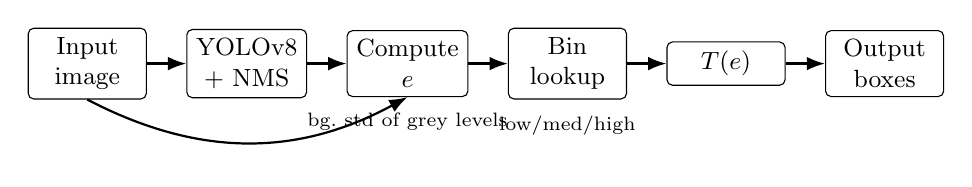
\begin{tikzpicture}[
      node distance=0.35cm and 0.5cm,
      box/.style={rectangle, draw, rounded corners=2pt,
                  minimum height=0.55cm, minimum width=1.5cm,
                  font=\small, align=center},
      arr/.style={-Latex, thick}
    ]
    \node[box] (img)   {Input\\image};
    \node[box, right=of img] (det) {YOLOv8\\+ NMS};
    \node[box, right=of det] (prx) {Compute\\$e$};
    \node[box, right=of prx] (lut) {Bin\\lookup};
    \node[box, right=of lut] (thr) {$T(e)$};
    \node[box, right=of thr] (out) {Output\\boxes};
    \draw[arr] (img) -- (det);
    \draw[arr] (det) -- (prx);
    \draw[arr] (img.south) to[bend right=28] (prx.south);
    \draw[arr] (prx) -- (lut);
    \draw[arr] (lut) -- (thr);
    \draw[arr] (thr) -- (out);
    \node[below=0.08cm of prx, font=\scriptsize] {bg.\ std of grey levels};
    \node[below=0.08cm of lut, font=\scriptsize] {low/med/high};
  \end{tikzpicture}%
  }
  \caption{Inference pipeline. The detector and NMS are unchanged. The
           clutter proxy $e$ is computed from the input image outside the
           detector's own boxes, mapped to a bin, and the per-bin threshold
           $T(e)$ gates the score-sorted detection list.}
  \label{fig:pipeline}
\end{figure}

\subsection{Setting: Training Is Untouched}
\label{sec:setting}
\linelabel{ln:train}Let $f$ be a trained detector that, after NMS, returns boxes with scores
$s_i\in[0,1]$ for image $x$. Deployment keeps $\{i: s_i\ge T\}$ for one
global $T$. We replace $T$ by $T(e(x))$, where $e(x)$ is a scalar clutter
statistic of $x$. The detector is trained once with its standard loss and
model selection; $T(\cdot)$ is fitted afterwards on cached predictions of a
held-out calibration split and is never used during training. Hence it
affects neither the loss nor the selected checkpoint (Fig.~\ref{fig:pipeline}).\linelabel{ln:trainend}

\subsection{Clutter Proxy}
\label{sec:proxy}
\linelabel{ln:dn}Both benchmarks are distributed as 8-bit grey-scale images. We compute
$e$ from the stored digital numbers (DNs) $g(p)\in\{0,\dots,255\}$
(PIL ``L'' conversion), not from calibrated amplitude, intensity,
log-intensity/dB values, or the normalised YOLO input tensor; no
resizing, normalisation, clipping, or radiometric calibration precedes
the computation of $e$.\linelabel{ln:dnend} Let $\mathcal{D}$ be the set
of detector boxes with $s_i\ge 0.25$ (the mask gate), each dilated by $k$
pixels, and $\Omega=\{p\notin\bigcup\mathcal{D}\}$ the remaining
background pixels. Then
\begin{equation}
  e(x)=\Big(\tfrac{1}{|\Omega|}\textstyle\sum_{p\in\Omega}\big(g(p)-\bar g_\Omega\big)^2\Big)^{1/2},
  \label{eq:proxy}
\end{equation}
with $\Omega$ replaced by the full image if $|\Omega|<100$. We use $k{=}8$
for $800\times800$ SARDet-100K tiles\linelabel{ln:k} and $k{=}3$ for $256\times256$
SAR-Ship-Dataset tiles ($\approx3\%$ of tile width) to exclude side-lobe
and wake pixels adjacent to ships; Sec.~\ref{sec:robust} shows the result is
insensitive to $k\in[0,16]$. Ground-truth boxes are never used.\linelabel{ln:kend}

\textit{Why the standard deviation.}\linelabel{ln:rayl}
For fully developed speckle the amplitude is Rayleigh distributed with
$\sigma\propto\mu$; high-resolution or high-sea-state clutter is better
described by compound (K, Weibull, log-normal) models with heavier
tails~\cite{ward1981,oliver2004}. Under all of these, the dispersion of
background amplitude increases monotonically with the clutter scale, which
is the only property the proxy relies on --- we do not assume Rayleigh
statistics. The same dispersion statistic is estimated locally by CA-CFAR
detectors~\cite{finn1968}; we estimate it once per image. $e$ needs no
external data (e.g.\ ERA5~\cite{hersbach2020}) and costs $<2$~ms per
$800\times800$ tile on one CPU core.\linelabel{ln:raylend}

\subsection{Binning and Per-Bin Calibration}
\label{sec:calib}
On the calibration split, $e$ is tertile-binned into
$\mathcal{B}=\{\text{low},\text{medium},\text{high}\}$. Quantile bins are
preferred to equal-width bins because $e$ is strongly right-skewed (the
\linelabel{ln:bins}99th percentile is $\sim20\times$ the median), and tertiles give equal
support per bin: $2147$ images per bin on SARDet-100K and
$1460/1460/1461$ on SAR-Ship-Dataset (calibration), $2152/2144/2200$ and
$1515/1335/1531$ on the test splits. \linelabel{ln:single}Both benchmarks are single-class (ship), so one threshold
per bin is fitted on the calibration images of bin $b$ by one of three
criteria:
\begin{align}
  \text{F1-balanced:}\quad & T_b=\arg\max_T \mathrm{F1}_b(T), \label{eq:f1}\\
  \text{FA budget:}\quad & T_b=\min\{T:\ \mathrm{FA}_b(T)\le\beta\}, \label{eq:fa}\\
  \text{Precision target:}\quad & T_b=\min\{T:\ \mathrm{P}_b(T)\ge\pi\}, \label{eq:prec}
\end{align}
where $\mathrm{FA}_b$ is the number of false alarms per image. Because
recall is non-increasing in $T$, Eqs.~\eqref{eq:fa}--\eqref{eq:prec} give
the highest recall that meets the constraint; Eq.~\eqref{eq:prec} is
identical to the recall-biased criterion of the previous version. The
\emph{global} counterpart of each criterion applies the same rule to the
whole calibration split. Targets are fixed before evaluation:
$\beta\in\{0.5,1,2\}\times$ the calibration false-alarm rate of
$T{=}0.40$ ($0.116$ / $0.121$ per image on SARDet-100K /
SAR-Ship-Dataset), i.e.\ the production budget, halved and doubled;
$\pi\in\{0.85,0.90,0.95\}$. $T$ is scanned on
$\{0.05,0.075,\dots,0.85\}$ for Eq.~\eqref{eq:f1} and in steps of $0.005$
for Eqs.~\eqref{eq:fa}--\eqref{eq:prec}. $T_b$ may fall above \emph{or}
below the global baseline in any bin.\linelabel{ln:dir}

\subsection{Functional Forms and Inference}
\linelabel{ln:derived}\textbf{Piecewise-constant}: $T(e)=T_{b(e)}$ (a three-entry look-up table
with two edges). \textbf{Linear}: $T(e)=a\,e+b$, least-squares fitted
through the three anchors (median $e$ of each bin, $T_b$) and clipped to
$[0.05,0.9]$. At inference, detections with $s_i<T(e)$ are discarded. For
SAR-Ship-Dataset with Eq.~\eqref{eq:f1} the fitted values are: edges
$e{=}2.62, 17.87$; $T_b=(0.425, 0.475, 0.550)$; $a{=}0.0033$, $b{=}0.434$
(SARDet-100K values in Table~\ref{tab:main}).\linelabel{ln:derivedend}

\subsection{Evaluation Protocol}
\label{sec:protocol}
\linelabel{ln:ap}All metrics are computed on the \emph{delivered} detection set
$\{i:s_i\ge T(e)\}$. P, R, F1, and FA per image are single operating-point
values. ``AP'' denotes AP@0.5 with 101-point interpolation computed on the
gated list ranked by the \emph{original} scores (gated AP); it is bounded
by the ungated AP and is non-increasing in $T$, so it can only credit a
policy that \emph{lowers} the threshold, whereas F1 credits both
directions.\linelabel{ln:apend} Clutter invariance is measured on the test split, per true
clutter stratum, by the \emph{spread} $\max_b-\min_b$ of FA per image (or
precision), and by the \emph{worst-stratum load} $\max_b\mathrm{FA}_b/\beta$
(or the largest precision shortfall below $\pi$). Uncertainty is given by
200 bootstrap resamples of test images within strata, and a
random-binning placebo (20 random partitions with the true bin sizes,
thresholds re-fitted each time) tests whether any three-way split would do
as well. \linelabel{ln:pfa}FA per image is an image-level, post-NMS
quantity, not the per-cell probability of false alarm $P_{\mathrm{FA}}$
of classical CFAR; the analogy concerns the operating goal, not the test
statistic.\linelabel{ln:pfaend}

% ---------------------------------------------------------------
\section{Experiments}
\label{sec:experiments}
% ---------------------------------------------------------------

\subsection{Setup}
\linelabel{ln:data}\textbf{Datasets.}
\textit{SARDet-100K}~\cite{sardet100k}: we use the official splits
restricted to images containing at least one ship (calibration on
\textsc{val}, 6441 images; report on \textsc{test}, 6496).
\textit{SAR-Ship-Dataset}~\cite{sarship2019}: 43{,}819 tiles of
$256\times256$ px from GF-3 and Sentinel-1, single class, deterministic
80/10/10 split (calibration on the 10\,\% validation split, 4381
images; report on the 10\,\% test split, 4381).
\textbf{Detector.} YOLOv8s~\cite{yolov8}, 100 epochs, seed 42, standard
Ultralytics recipe and checkpoint selection, one model per dataset.
Ungated test AP@0.5 is 0.940 (SARDet-100K) and 0.962
(SAR-Ship-Dataset); at the production default $T{=}0.40$ the gated AP is
0.891 / 0.928. Only the gate is modified by our method.
\linelabel{ln:code}\textbf{Code} (training, caching, calibration, all controls and per-image
$e$ values) is available at \TBD{\url{https://github.com/<user>/eat-sar}}.

\subsection{Clutter-Invariant False-Alarm Operation}
\label{sec:cfar}
\linelabel{ln:cfar}Fig.~\ref{fig:cfar} shows the per-stratum false-alarm rate and precision
on the test splits when a global threshold and the conditioned policy are
fitted to the same target. With the production budget, the global
threshold ($T{=}0.405$ / $0.40$) leaves the false alarms concentrated in
high clutter ($0.035$, $0.131$, $0.228$ per image on SARDet-100K;
$0.044$, $0.100$, $0.226$ on SAR-Ship-Dataset). The conditioned policy
spends the same budget evenly ($0.135$, $0.167$, $0.124$; $0.118$,
$0.116$, $0.113$) with $T_b=(0.105, 0.32, 0.56)$ and
$(0.065, 0.335, 0.615)$ --- again rising with clutter. The worst-stratum
load drops from $1.97$ to $1.44$ times the budget on SARDet-100K and from
$1.87$ to $0.97$ on SAR-Ship-Dataset; on SARDet-100K all policies exceed
the budget because the test split is harder than the calibration split
($0.135$ vs.\ $0.116$ FA per image at $T{=}0.40$). Precision targets behave
alike: at $\pi{=}0.90$ the global threshold delivers $84$--$96\,\%$
across strata, the conditioned policy $86$--$90\,\%$.

Table~\ref{tab:cfar} lists all twelve pre-specified settings. The spread
falls by $3.1$--$4.5\times$ on SARDet-100K and $2.8$--$41\times$ on
SAR-Ship-Dataset; in every setting the bootstrap 95\,\% interval of the
reduction excludes zero, and so does that of the worst-stratum load in
10 of 12 settings (the exceptions are SARDet-100K at $\pi{=}0.90$ and
$0.95$). The random-binning placebo never reduces the spread: its mean is
within $2.2\,\%$ of the global threshold's in all twelve settings, and the
conditioned policy lies $23$--$65$ placebo standard deviations below it.
Clutter invariance is therefore produced by conditioning on $e$, not by
fitting three thresholds instead of one.

Uniformity has a price, which we report. The overall F1 changes by
$-1.56$ to $+0.55$~pp relative to the global threshold at the same
target (Table~\ref{tab:cfar}); at the production budget recall falls by
$1.5$ / $2.2$~pp. Spreading the budget evenly lowers the gate in low
clutter, where almost no ships remain to be recovered (recall already
$\ge0.97$), and raises it in high clutter, where some ships are lost. A
clutter-invariant false-alarm rate is thus a different operating
objective from maximal F1, chosen when the cost of verifying detections
must not depend on the clutter conditions.\linelabel{ln:cfarend}

\begin{figure}[t]
  \centering
  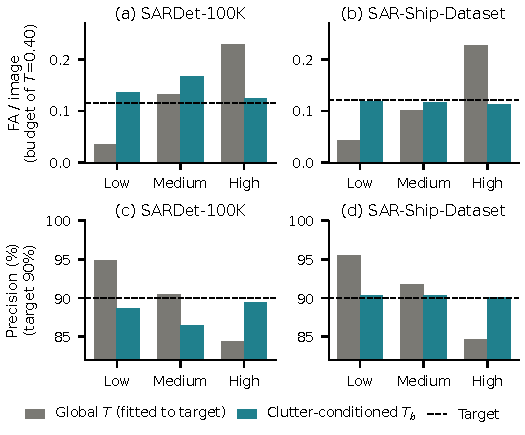
\includegraphics[width=\columnwidth]{figs/fig_cfar.pdf}
  \caption{False alarms per image (a, b) and precision (c, d) per clutter
           stratum on the test splits, for a global threshold and the
           clutter-conditioned policy fitted to the same target on the
           calibration split: (a, b) the false-alarm budget of $T{=}0.40$
           (Eq.~\eqref{eq:fa}); (c, d) $\pi{=}0.90$ (Eq.~\eqref{eq:prec}).}
  \label{fig:cfar}
\end{figure}

\begin{table}[t]
\centering
\caption{Clutter invariance at matched targets (test splits). Spread:
$\max_b-\min_b$ over the true clutter strata of FA per image (rows
$\beta$) or of precision in pp (rows $\pi$), for the global threshold (G)
and the conditioned policy (C). $\Delta$F1: C minus G, in pp. Bootstrap
95\,\% intervals of G$-$C exclude zero in all rows; the placebo spread is
within 2.2\,\% of G in all rows.}
\label{tab:cfar}
\footnotesize
\setlength{\tabcolsep}{3.2pt}
\begin{tabular}{l ccr ccr}
\toprule
 & \multicolumn{3}{c}{SARDet-100K} & \multicolumn{3}{c}{SAR-Ship-Dataset} \\
\cmidrule(lr){2-4}\cmidrule(lr){5-7}
Target & G & C & $\Delta$F1 & G & C & $\Delta$F1 \\
\midrule
$\beta{=}0.5\times$ & 0.099 & 0.026 & $-$1.37 & 0.092 & 0.022 & $-$1.56 \\
$\beta{=}1\times$   & 0.193 & 0.043 & $-$1.12 & 0.182 & 0.0045 & $-$0.85 \\
$\beta{=}2\times$   & 0.415 & 0.133 & $-$0.13 & 0.370 & 0.123 & $+$0.55 \\
$\pi{=}0.85$        & 15.7  & 3.8   & $-$0.03 & 15.0  & 5.4   & $+$0.16 \\
$\pi{=}0.90$        & 10.4  & 3.0   & $-$0.70 & 10.8  & 0.3   & $-$0.32 \\
$\pi{=}0.95$        & 6.2   & 1.8   & $-$0.86 & 5.9   & 1.6   & $-$1.13 \\
\bottomrule
\end{tabular}
\end{table}

% ------ Table I (full width) ------
\begin{table*}[t]
\centering
\caption{Global threshold vs.\ F1-balanced environment-conditioned
thresholding (Eq.~\eqref{eq:f1}) on the test splits (images with $\ge1$
ship). $T_b$: fitted per-bin threshold (calibration split). P/R/F1: single
operating point. AP: gated AP@0.5 (Sec.~\ref{sec:protocol}). $\Delta$ in
percentage points vs.\ the baseline row of the same bin. Bin edges
(calibration tertiles of $e$): SARDet-100K 4.5/20.0, SAR-Ship-Dataset
2.6/17.9.}
\label{tab:main}
\small
\setlength{\tabcolsep}{4pt}
\begin{tabular}{l l l c c c c r c r}
\toprule
Dataset & Strategy & Bin & $T_b$ & P & R & F1 & $\Delta$F1 & AP & $\Delta$AP \\
\midrule
SARDet-100K & Baseline ($T{=}0.40$) & All            & 0.40 & 0.917 & 0.908 & 0.912 &      -- & 0.891 &      -- \\
            &                       & Low-clutter    & 0.40 & 0.968 & 0.978 & 0.973 &      -- & 0.967 &      -- \\
            &                       & Medium-clutter & 0.40 & 0.923 & 0.921 & 0.922 &      -- & 0.913 &      -- \\
            &                       & High-clutter   & 0.40 & 0.884 & 0.859 & 0.872 &      -- & 0.835 &      -- \\
\addlinespace[2pt]
            & Adaptive F1           & All            &    -- & 0.927 & 0.900 & 0.913 &   +0.08 & 0.891 & $-$0.00 \\
            &                       & Low-clutter    & 0.400 & 0.968 & 0.978 & 0.973 &   +0.00 & 0.967 &   +0.00 \\
            &                       & Medium-clutter & 0.425 & 0.928 & 0.917 & 0.923 &   +0.07 & 0.904 & $-$0.91 \\
            &                       & High-clutter   & 0.450 & 0.902 & 0.845 & 0.872 &   +0.07 & 0.826 & $-$0.89 \\
\midrule
SAR-Ship-Dataset & Baseline ($T{=}0.40$) & All        & 0.40 & 0.912 & 0.949 & 0.930 &      -- & 0.928 &      -- \\
            &                       & Low-clutter    & 0.40 & 0.960 & 0.983 & 0.971 &      -- & 0.977 &      -- \\
            &                       & Medium-clutter & 0.40 & 0.930 & 0.968 & 0.948 &      -- & 0.949 &      -- \\
            &                       & High-clutter   & 0.40 & 0.869 & 0.913 & 0.891 &      -- & 0.888 &      -- \\
\addlinespace[2pt]
            & Adaptive F1           & All            &    -- & 0.935 & 0.929 & 0.932 &   +0.22 & 0.910 & $-$1.84 \\
            &                       & Low-clutter    & 0.425 & 0.962 & 0.980 & 0.971 & $-$0.04 & 0.977 &   +0.00 \\
            &                       & Medium-clutter & 0.475 & 0.943 & 0.959 & 0.951 &   +0.26 & 0.940 & $-$0.93 \\
            &                       & High-clutter   & 0.550 & 0.911 & 0.875 & 0.893 &   +0.21 & 0.853 & $-$3.53 \\
\bottomrule
\end{tabular}
\end{table*}

\subsection{F1-Balanced Policy and Controls}
\label{sec:controls}
\linelabel{ln:ctrl}Table~\ref{tab:main} reports the F1-balanced policy. The fitted
thresholds are $T_b-0.40=(+0.00,+0.025,+0.05)$ on SARDet-100K and
$(+0.025,+0.075,+0.15)$ on SAR-Ship-Dataset\linelabel{ln:hi}: the gate rises
monotonically with clutter, i.e.\ clutter-induced false alarms dominate
the detector's errors in the high bin (SAR-Ship-Dataset: $+4.2$~pp P for
$-3.8$~pp R).\linelabel{ln:hiend} Because the policy only raises the gate, gated AP can only
fall (Sec.~\ref{sec:protocol}). The aggregate F1 gain, $+0.08$ /
$+0.22$~pp, is not attributable to clutter conditioning
(Table~\ref{tab:controls}). \linelabel{ln:ctrlA}(A) A single validation-optimal threshold
$T^{*}{=}0.45$ / $0.475$ already gives $+0.06$ / $+0.30$~pp. (B) The
random-binning placebo gives $+0.06$ / $+0.23$~pp, as much as the true
binning (placebo $z{=}0.9$ / $-0.02$). (C) A global threshold matching the
policy's recall or number of detections lands within $0.01$--$0.08$~pp F1.
(D) Per-bin thresholds fitted on the test split itself reach only
$+0.10$ / $+0.36$~pp, because F1($T$) is nearly flat near its optimum
(Fig.~\ref{fig:curves}). On these well-trained detectors, therefore, no
per-bin policy can raise aggregate F1 materially, and the F1 gain that
exists comes from using a validation split at all. The linear form
behaves like the piecewise one ($0.913$ vs.\ $0.913$; $0.928$ vs.\
$0.932$).\linelabel{ln:ctrlend}

\begin{table}[t]
\centering
\caption{Aggregate controls for the F1-balanced criterion: overall test
$\Delta$F1 / $\Delta$AP (pp) vs.\ the baseline $T{=}0.40$. Placebo: mean
over 20 random binnings.}
\label{tab:controls}
\footnotesize
\setlength{\tabcolsep}{3.5pt}
\begin{tabular}{l c c c c}
\toprule
 & \multicolumn{2}{c}{SARDet-100K} & \multicolumn{2}{c}{SAR-Ship-Dataset} \\
\cmidrule(lr){2-3}\cmidrule(lr){4-5}
Policy & $\Delta$F1 & $\Delta$AP & $\Delta$F1 & $\Delta$AP \\
\midrule
(A) Val-optimal global $T^{*}$          & +0.06 & $-$0.92 & +0.30 & $-$0.92 \\
(B) Random bins (placebo)               & +0.06 & $-$0.32 & +0.23 & $-$1.10 \\
(C) Global $T$ at same \#detections     & +0.09 & $-$0.00 & +0.30 & $-$0.92 \\
Adaptive F1, linear                     & +0.05 & $-$0.92 & $-$0.24 & $-$2.78 \\
\textbf{Adaptive F1, piecewise}         & \textbf{+0.08} & \textbf{$-$0.00} & \textbf{+0.22} & \textbf{$-$1.84} \\
(D) Oracle: per-bin $T$ fit on test     & +0.10 & $-$0.92 & +0.36 & $-$0.92 \\
\bottomrule
\end{tabular}
\end{table}

\subsection{Robustness of the Calibration}
\label{sec:robust}
\linelabel{ln:cv}\emph{10-fold cross-validation.} Each fold re-fits edges and $T_b$
(Eq.~\eqref{eq:f1}) on 90\,\% of the calibration split, stratified by
tertile, and is scored on the held-out 10\,\% and on the test split. The
thresholds are stable ($T_{\text{high}}{=}0.550\pm0.000$
SAR-Ship-Dataset, $0.440\pm0.013$ SARDet-100K), the sign of
$T_{\text{high}}-0.40$ never flips, and the test $\Delta$F1 is
$+0.06\pm0.03$ / $+0.24\pm0.03$~pp, positive in 10/10 folds.\linelabel{ln:cvend}
\linelabel{ln:ksweep}\emph{Dilation $k$.} Re-computing $e$ with $k\in\{0,3,5,8,12,16\}$
(SARDet-100K) and $\{0,1,2,3,5,8\}$ (SAR-Ship-Dataset) keeps the rank
correlation with the default $e$ above $0.99$ and the overall test
$\Delta$F1 within $+0.08$ / $+0.22$--$0.28$~pp; even $k{=}0$ changes it by
at most $0.03$~pp. We fix three bins throughout; the linear form, a single
continuous fit, behaves like the piecewise one.\linelabel{ln:ksweepend}

\subsection{Is $e$ a Valid Clutter Proxy?}
\label{sec:proxyval}
\linelabel{ln:proxy}Neither benchmark provides acquisition time or footprint, so $e$
cannot be matched to an external sea-state product such as
ERA5~\cite{hersbach2020}; $e$ is therefore an image-level clutter
proxy, not a physical sea-state estimate. We validate it against
classical clutter statistics on the same background pixels of the
calibration splits (SARDet-100K / SAR-Ship-Dataset). $e$ is rank-correlated with the
mean backscatter $\mu$ ($\rho{=}0.92$ / $0.91$), histogram entropy
($0.94$ / $0.94$), and the robust spread $p_{99}-\text{median}$
($0.97$ / $0.96$): high-$e$ scenes are brighter and spikier. The median
$\sigma/\mu$ is $0.87$ / $0.94$ in the low bin and $0.66$ / $0.77$ in the
high bin, $1.3$--$1.8$ times the Rayleigh value $0.523$ in every stratum,
so no stratum is fully developed speckle --- which the proxy tolerates
(Sec.~\ref{sec:proxy}). The method-of-moments K-shape estimate is only
weakly related to $e$ ($\rho{=}0.31$ / $0.42$) and degenerate in the low
bin, so we do not rely on it. Finally, $e$ computed with detector boxes
agrees with a ground-truth-masked version to $\rho\ge0.99$ and assigns
$98.3$ / $96.6$\,\% of images to the same tertile, so detector errors do
not corrupt the proxy.\linelabel{ln:proxyend}

\subsection{Transfer Across Datasets and Sensors}
\label{sec:transfer}
\linelabel{ln:transfer}SARDet-100K aggregates several sensors and SAR-Ship-Dataset is GF-3 and
Sentinel-1, each with its own 8-bit scaling. Applying the SARDet-100K
edges and $T_b$ (Eq.~\eqref{eq:f1}) unchanged to SAR-Ship-Dataset gives
$+0.14$~pp F1, within $0.08$~pp of the in-domain fit; re-estimating only
the edges as tertiles of $e$ on the \emph{unlabelled} target images gives
$+0.13$~pp. The reverse direction loses at most $0.2$~pp F1 ($-0.11$ /
$-0.14$ vs.\ $+0.08$~pp in-domain). The monotone direction of the
correction is preserved both ways.\linelabel{ln:transferend}

\begin{figure*}[!t]
  \centering
  \begin{subfigure}[t]{0.245\textwidth}
    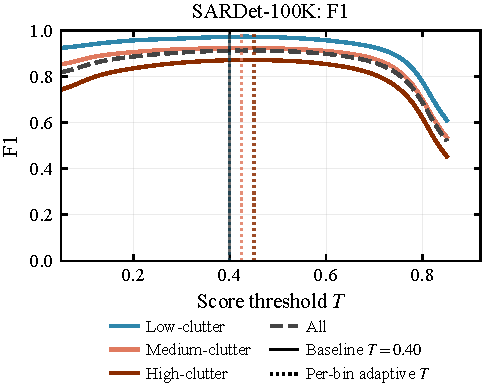
\includegraphics[width=\linewidth]{figs/fig_curves_sardet_f1.pdf}
    \caption{SARDet-100K, F1}
  \end{subfigure}\hfill
  \begin{subfigure}[t]{0.245\textwidth}
    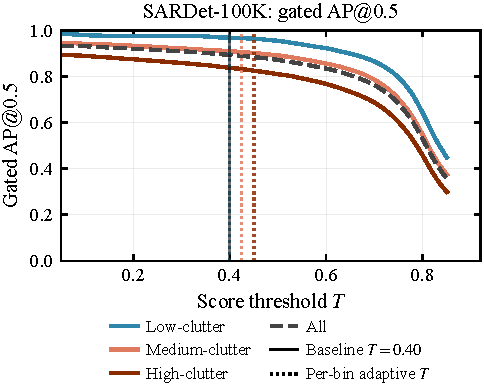
\includegraphics[width=\linewidth]{figs/fig_curves_sardet_map.pdf}
    \caption{SARDet-100K, gated AP}
  \end{subfigure}\hfill
  \begin{subfigure}[t]{0.245\textwidth}
    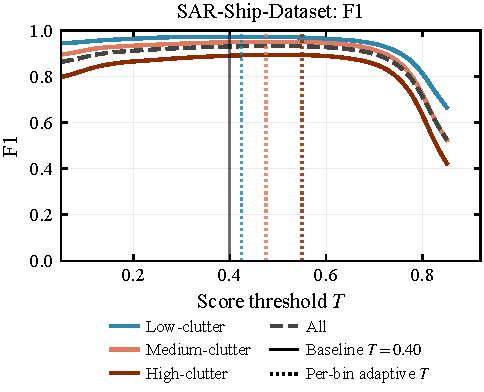
\includegraphics[width=\linewidth]{figs/fig_curves_sarship_f1.pdf}
    \caption{SAR-Ship-Dataset, F1}
  \end{subfigure}\hfill
  \begin{subfigure}[t]{0.245\textwidth}
    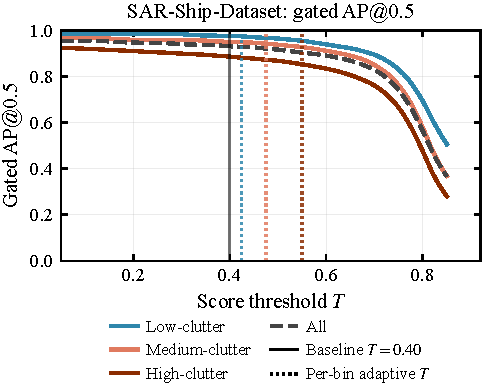
\includegraphics[width=\linewidth]{figs/fig_curves_sarship_map.pdf}
    \caption{SAR-Ship-Dataset, gated AP}
  \end{subfigure}
  \caption{F1 (a, c) and gated AP@0.5 (b, d) vs.\ score threshold $T$
           per clutter bin on the test splits. Solid vertical line: global
           baseline $T{=}0.40$; dotted: F1-balanced $T_b$ per bin (fitted on
           the calibration split). F1($T$) is nearly flat near its optimum,
           especially in low clutter, which bounds every per-bin policy
           (Sec.~\ref{sec:controls}).}
  \label{fig:curves}
\end{figure*}

% ---------------------------------------------------------------
\section{Conclusion}
\label{sec:conclusion}
% ---------------------------------------------------------------
\linelabel{ln:concl}A single global score threshold gives a deep SAR ship detector a
false-alarm rate that depends on the clutter: 5--6 times higher in the
high- than in the low-clutter tertile on two benchmarks. Conditioning the
post-NMS gate on a per-image clutter statistic, calibrated offline to a
false-alarm budget or a precision target, yields a CFAR-inspired,
more clutter-invariant false-alarm operating point:
across twelve pre-specified settings the cross-stratum spread falls by
$2.8$--$41\times$ with bootstrap intervals excluding zero, while a global
threshold fitted to the same target and a random-binning placebo leave it
unchanged; the price is at most $1.6$~pp F1. The same controls show that
an F1-maximising variant gains no more than a validation-tuned global
threshold on well-trained detectors. The policy is two edges and three
scalars, costs $<2$~ms per tile, needs no retraining or metadata, and
transfers across sensors after label-free quantile normalisation. Future
work includes validation against co-registered sea-state data,
per-pixel false-alarm control, and multi-class detection.\linelabel{ln:conclend}

\bibliographystyle{IEEEtran}
\bibliography{refs}

\end{document}
